\documentclass[a4paper, 14pt]{extarticle}

% Поля
%--------------------------------------
\usepackage{geometry}
\geometry{a4paper,tmargin=2cm,bmargin=2cm,lmargin=3cm,rmargin=1cm}
%--------------------------------------


%Russian-specific packages
%--------------------------------------
\usepackage[T2A]{fontenc}
\usepackage[utf8]{inputenc} 
\usepackage[english, main=russian]{babel}
%--------------------------------------

\usepackage{textcomp}

% Красная строка
%--------------------------------------
\usepackage{indentfirst}               
%--------------------------------------             


%Graphics
%--------------------------------------
\usepackage{graphicx}
\graphicspath{ {./images/} }
\usepackage{wrapfig}
%--------------------------------------

% Полуторный интервал
%--------------------------------------
\linespread{1.3}                    
%--------------------------------------

%Выравнивание и переносы
%--------------------------------------
% Избавляемся от переполнений
\sloppy
% Запрещаем разрыв страницы после первой строки абзаца
\clubpenalty=10000
% Запрещаем разрыв страницы после последней строки абзаца
\widowpenalty=10000
%--------------------------------------

%Списки
\usepackage{enumitem}

%Подписи
\usepackage{caption} 

%Гиперссылки
\usepackage{hyperref}

\hypersetup {
	unicode=true
}

%Рисунки
%--------------------------------------
\DeclareCaptionLabelSeparator*{emdash}{~--- }
\captionsetup[figure]{labelsep=emdash,font=onehalfspacing,position=bottom}
%--------------------------------------

\usepackage{tempora}

%Листинги
%--------------------------------------
\usepackage{listings}
\lstset{
  basicstyle=\ttfamily\footnotesize, 
  %basicstyle=\footnotesize\AnkaCoder,        % the size of the fonts that are used for the code
  breakatwhitespace=false,         % sets if automatic breaks shoulbd only happen at whitespace
  breaklines=true,                 % sets automatic line breaking
  captionpos=t,                    % sets the caption-position to bottom
  inputencoding=utf8,
  frame=single,                    % adds a frame around the code
  keepspaces=true,                 % keeps spaces in text, useful for keeping indentation of code (possibly needs columns=flexible)
  keywordstyle=\bf,       % keyword style
  numbers=left,                    % where to put the line-numbers; possible values are (none, left, right)
  numbersep=5pt,                   % how far the line-numbers are from the code
  xleftmargin=25pt,
  xrightmargin=25pt,
  showspaces=false,                % show spaces everywhere adding particular underscores; it overrides 'showstringspaces'
  showstringspaces=false,          % underline spaces within strings only
  showtabs=false,                  % show tabs within strings adding particular underscores
  stepnumber=1,                    % the step between two line-numbers. If it's 1, each line will be numbered
  tabsize=2,                       % sets default tabsize to 8 spaces
  title=\lstname                   % show the filename of files included with \lstinputlisting; also try caption instead of title
}
%--------------------------------------

%%% Математические пакеты %%%
%--------------------------------------
\usepackage{amsthm,amsfonts,amsmath,amssymb,amscd}  % Математические дополнения от AMS
\usepackage{mathtools}                              % Добавляет окружение multlined
\usepackage[perpage]{footmisc}
%--------------------------------------

%--------------------------------------
%			НАЧАЛО ДОКУМЕНТА
%--------------------------------------

\begin{document}

%--------------------------------------
%			ТИТУЛЬНЫЙ ЛИСТ
%--------------------------------------
\begin{titlepage}
\thispagestyle{empty}
\newpage


%Шапка титульного листа
%--------------------------------------
\vspace*{-60pt}
\hspace{-65pt}
\begin{minipage}{0.3\textwidth}
\hspace*{-20pt}\centering

\includegraphics[width=\textwidth]{emblem}
\end{minipage}
\begin{minipage}{0.67\textwidth}\small \textbf{
\vspace*{-0.7ex}
\hspace*{-6pt}\centerline{Министерство науки и высшего образования Российской Федерации}
\vspace*{-0.7ex}
\centerline{Федеральное государственное бюджетное образовательное учреждение }
\vspace*{-0.7ex}
\centerline{высшего образования}
\vspace*{-0.7ex}
\centerline{<<Московский государственный технический университет}
\vspace*{-0.7ex}
\centerline{имени Н.Э. Баумана}
\vspace*{-0.7ex}
\centerline{(национальный исследовательский университет)>>}
\vspace*{-0.7ex}
\centerline{(МГТУ им. Н.Э. Баумана)}}
\end{minipage}
%--------------------------------------

%Полосы
%--------------------------------------
\vspace{-25pt}
\hspace{-35pt}\rule{\textwidth}{2.3pt}

\vspace*{-20.3pt}
\hspace{-35pt}\rule{\textwidth}{0.4pt}
%--------------------------------------

\vspace{1.5ex}
\hspace{-35pt} \noindent \small ФАКУЛЬТЕТ\hspace{80pt} <<Информатика и системы управления>>

\vspace*{-16pt}
\hspace{47pt}\rule{0.83\textwidth}{0.4pt}

\vspace{0.5ex}
\hspace{-35pt} \noindent \small КАФЕДРА\hspace{50pt} <<Теоретическая информатика и компьютерные технологии>>

\vspace*{-16pt}
\hspace{30pt}\rule{0.866\textwidth}{0.4pt}
  
\vspace{11em}

\begin{center}
\Large {\bf Лабораторная работа № 10} \\ 
\large {\bf по курсу <<Языки и методы программирования>>} \\
\large <<Реализация итераторов на языке C++>> 
\end{center}\normalsize

\vspace{8em}


\begin{flushright}
  {Студент группы ИУ9-21Б Горбунов А. Д. \hspace*{15pt}\\ 
  \vspace{2ex}
  Преподаватель Посевин Д. П.\hspace*{15pt}}
\end{flushright}

\bigskip

\vfill
 

\begin{center}
\textsl{Москва 2023}
\end{center}
\end{titlepage}
%--------------------------------------
%		КОНЕЦ ТИТУЛЬНОГО ЛИСТА
%--------------------------------------

\renewcommand{\ttdefault}{pcr}

\setlength{\tabcolsep}{3pt}
\newpage
\setcounter{page}{2}

\section{Задание}\label{Sect::task}
    Строка, составленная из латинских букв, с константным однонаправленным итератором по максимальным «правильным» подстрокам.
    
    «Правильная» подстрока должна содержать либо исключительно гласные, либо исключительно согласные буквы.
\section{Результаты}\label{Sect::res}

Исходный код программы представлен в листинге~\ref{lst:code1}, ~\ref{lst:code2}, ~\ref{lst:code3}

\begin{figure}[!htb]
\begin{lstlisting}[language={c++},caption={main.cpp},label={lst:code1}]
#include "Substrings.h"
using namespace std;

int main() {
    Substrings s1("feegeeeozd UAIEOoeegreeju  uqwertyuiopasdfghjklzxcvbnm");
    for (Substrings::Iterator it = s1.begin(); it != s1.end(); ++it) {
        cout << *it << endl;
    }
    cout<<endl;
    Substrings s2("ee eeeo UAIEOoee ee uu e uio a");
    for (Substrings::Iterator it = s2.begin(); it != s2.end(); ++it) {
        cout << *it << endl;
    }
    cout<<endl;
    Substrings s3("dOuBlE fReE ");
    for (Substrings::Iterator it = s3.begin(); it != s3.end(); ++it) {
        cout << *it << endl;
    }
    return 0;
}
\end{lstlisting}
\end{figure}

\begin{figure}[!htb]
\begin{lstlisting}[language={c++},caption={Substrings.h},label={lst:code2}]
#include <iostream>
#include <string>
#include <iterator>
using namespace std;
class Substrings {
public:
    Substrings(const string& str) : str_(str) {}
    class Iterator : public iterator<forward_iterator_tag, string> {
    public:
        unsigned int start_pos = 0;
        string substring;

        Iterator(const string& str, unsigned int pos) : str_(str), start_pos(pos) {
            while (start_pos < str_.length() && !isVowel(str_[start_pos])) {
                start_pos++;
            }
            if (start_pos == str_.length()) {
                start_pos = 0;
                substring = "";
            }
            else {
                unsigned int end_pos = start_pos + 1;
                while (end_pos < str_.length() && isVowel(str_[end_pos])) {
                    end_pos++;
                }
                substring = str_.substr(start_pos, end_pos - start_pos);
                start_pos = end_pos;
            }
        }

        bool operator==(const Iterator& other) const {
            return start_pos == other.start_pos && substring == other.substring;
        }

        bool operator!=(const Iterator& other) const {
            return !(*this == other);
        }

        Iterator& operator++() {
            while (start_pos < str_.length() && !isVowel(str_[start_pos])) {
                start_pos++;
            }
            if (start_pos == str_.length()) {
                start_pos = 0;
                substring = "";
            }
            else {
                unsigned int end_pos = start_pos + 1;
                while (end_pos < str_.length() && isVowel(str_[end_pos])) {
                    end_pos++;
                }
                substring = str_.substr(start_pos, end_pos - start_pos);
                start_pos = end_pos;
            }
            return *this;
        }

        Iterator operator++(int) {
            Iterator temp = *this;
            ++(*this);
            return temp;
        }

        const string& operator*() const {
            return substring;
        }

    private:
        const string str_;

        bool isVowel(char c) const {
            return c == 'a' || c == 'e' || c == 'i' || c == 'o' || c == 'u' || c == 'A' || c == 'E' || c == 'I' || c == 'O' || c == 'U';
        }

    };
    Iterator begin() const {
        return Iterator(str_, 0);
    }
    Iterator end() const {
        return Iterator(str_, str_.length());
    }
private:
    const string str_;
};
\end{lstlisting}
\end{figure}


\begin{figure}[!htb]
\begin{lstlisting}[language={c++},caption={Substrings.h(продолжение)},label={lst:code3}]
        Iterator operator++(int) {
            Iterator temp = *this;
            ++(*this);
            return temp;
        }
        const string& operator*() const {
            return substring;
        }
    private:
        const string str_;

        bool isVowel(char c) const {
            return c == 'a' || c == 'e' || c == 'i' || c == 'o' || c == 'u' || c == 'A' || c == 'E' || c == 'I' || c == 'O' || c == 'U';
        }
    };
    Iterator begin() const {
        return Iterator(str_, 0);
    }
    Iterator end() const {
        return Iterator(str_, str_.length());
    }
private:
    const string str_;
};
\end{lstlisting}
\end{figure}

\begin{figure}[!htb]
Результат запуска представлен на рисунке ~\ref{fig:picture_1.png}, ~\ref{fig:picture_2.png}, ~\ref{fig:picture_3.png}
\end{figure}

\begin{figure}[!htb]
	\centering
	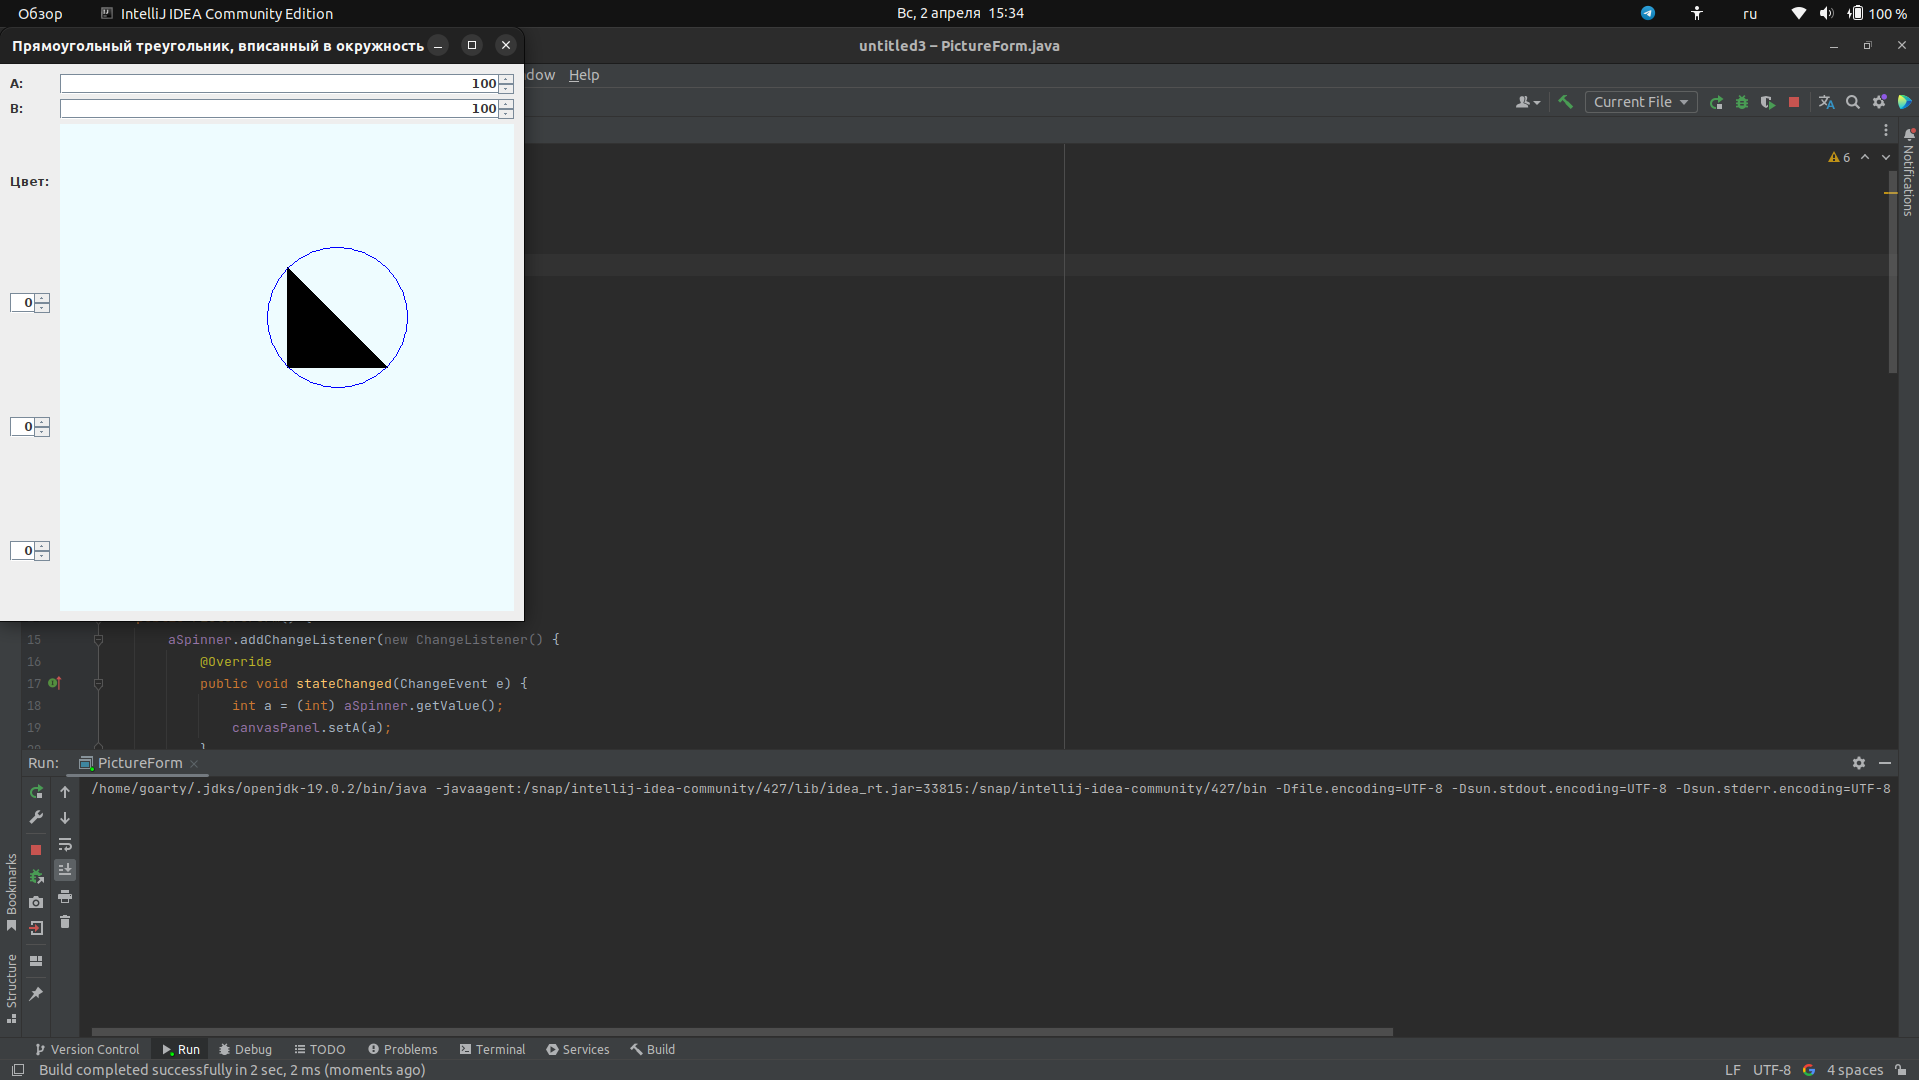
\includegraphics[width=0.8\textwidth]{picture_1.png}
\caption{Реализация main.cpp}
\label{fig:picture_1.png}
\end{figure}

\begin{figure}[!htb]
	\centering
	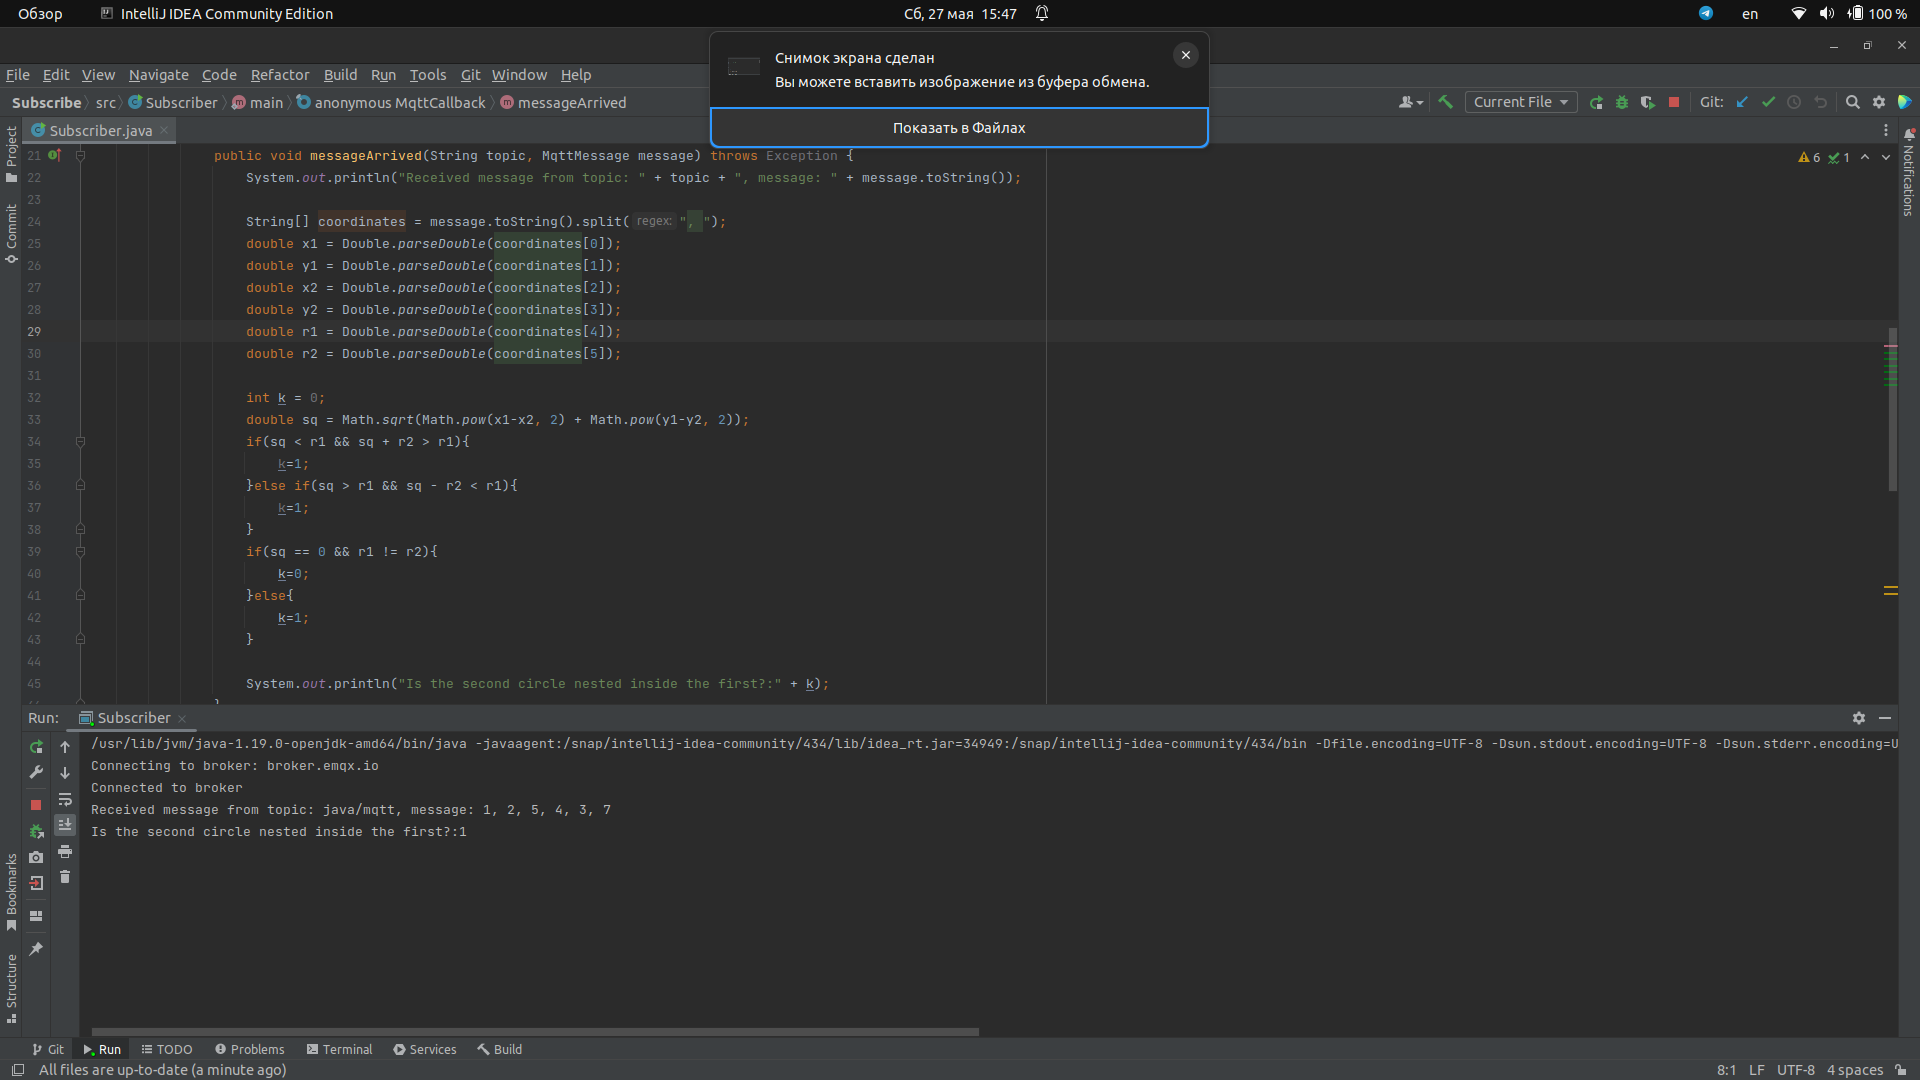
\includegraphics[width=0.8\textwidth]{picture_2.png}
\caption{Реализация Substrings.h}
\label{fig:picture_2.png}
\end{figure}

\begin{figure}[!htb]
	\centering
	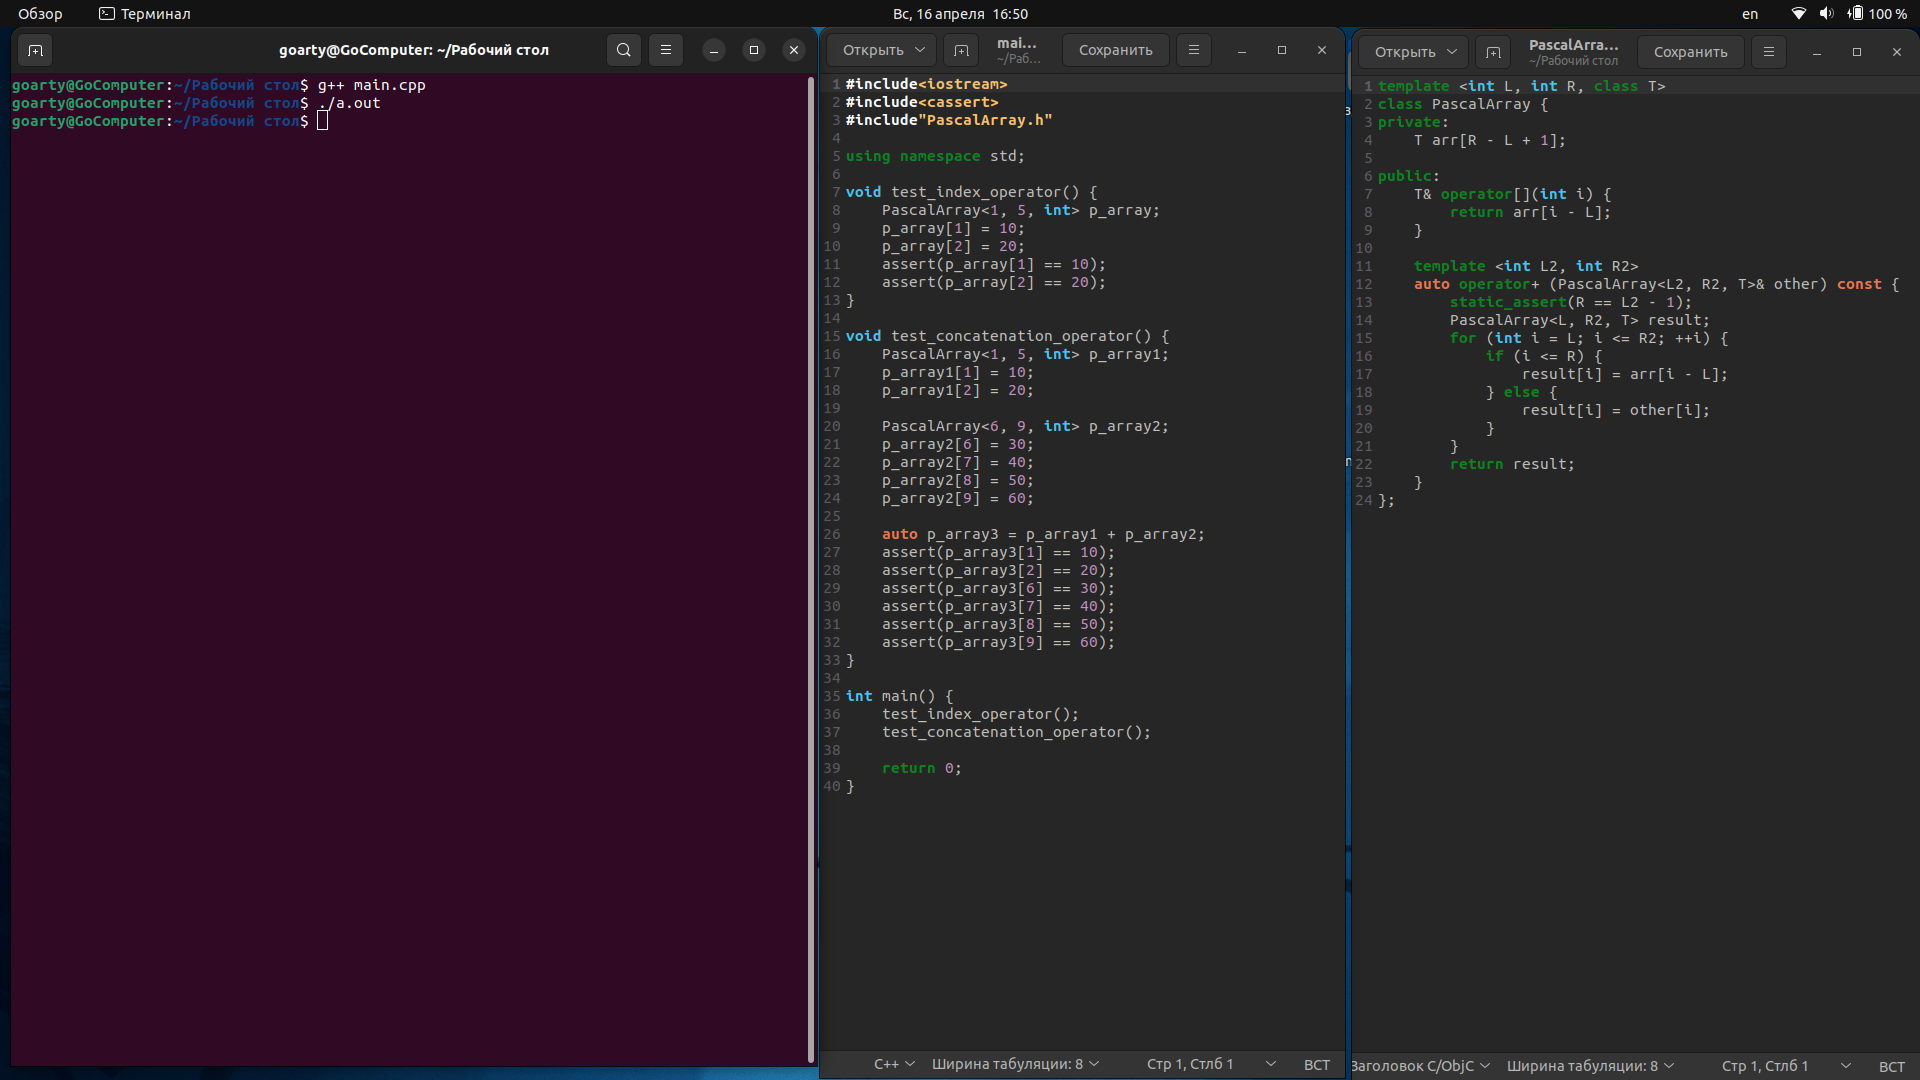
\includegraphics[width=0.8\textwidth]{picture_3.png}
\caption{Работа программы}
\label{fig:picture_3.png}
\end{figure}

\end{document}